

\section{Apresentação}
\subsection{Concedente}
% A Tecnologia da Informação (TI) busca oferecer aos usuários do Ministério da Cultura (MinC),
% assim como para os cidadãos brasileiros beneficiados pelas políticas culturais do Governo
% Federal, uma experiência inovadora e empolgante, onde a tecnologia possa ajudar a romper
% barreiras e facilitar a relação do Estado com o cidadão, gerando novas oportunidades de
% desenvolvimento social, econômico e cultural, além de estimular as inúmeras possibilidades de
% participação popular pelos meios digitais, modernizando assim também a nossa jovem
% democracia.

A missão da Coordenação Geral de Tecnologia da Informação-MinC, MinC/CGTEC, é oferecer para os usuários do Sistema Minc e para os cidadãos brasileiros uma
experiência tecnológica simples e intuitiva, por meio de ferramentas de gestão
participativa, de transparência de informações e da oferta de serviços digitais que facilitem
a relação do cidadão com as políticas públicas do Ministério da Cultura.

O Plano Diretor de Tecnologia da Informação e Comunicação - PDTI (2015-2017) apresenta a visão em 
tornar-se um modelo de gestão corporativa de TI pública, baseada em colaboração e
cooperação, com capacidade de atendimento de alta qualidade para seus usuários, com
foco no cidadão, com o apoio de soluções livres, métodos ágeis e governança participativa
de TI.

Um dos objetivos estratégicos do MinC/CGTEC é prospectar junto com universidades e
centros de P\&D novas formas de desenvolvimento de software. O presente projeto 
atende esse objetivo, no qual o papel da TI do Ministério da Cultura 
será o de orientar os objetivos e
desenvolvimento dessa cooperação, de forma a produzir pesquisa, inovação e
desenvolvimento aplicado para o aumento da colaboração no âmbito do setor
público. Nesse sentido, foi identificado na Universidade de Brasília a
possibilidade de formalizar uma parceria, de forma que o Laboratório Avançado
de Pesquisa e Desenvolvimento de Software (LAPPIS) da Faculdade UnB Gama (FGA)
possa elaborar pesquisas aplicadas e viabilizar o desenvolvimento e evolução
das plataformas mencionadas. A procura da parceria com o LAPPIS, nesse
contexto, é natural pelo compromisso e as experiências anteriores comprovadas
dos seus membros em ampliar o conhecimento do setor público e da sociedade no
uso de software livre.

% Dentre as diretrizes específicas propostas no PDTI para os anos 2015 à 2017 estão:
% 
% \begin{itemize}
%  \item Manter a transparência das suas ações e garantir a execução das deliberações
% do Comitê Estratégico de TI.
% \item Fomentar a participação das áreas na gestão dos projetos de TI.
% \item Melhorar a experiência e a satisfação dos usuários de TI do MinC.
% \item Fortalecer as iniciativas baseadas em software livre e dados abertos.
% \item Atuar em parceria com as áreas de negócio em busca de soluções conjuntas.
% \end{itemize}

% Na área de tecnologia, o Ministério da Cultura desenvolve sistemas para o 
% % fomento, incentivo cultural, e gestão e promoção de políticas públicas de cultura, liberado-os como software livre,
% e que são desenvolvidos em conjunto com comunidades de usuários e cidadãos interessados. 
% Há 27 projetos de software desenvolvidos e mantidos pela equipe do Ministério da Cultura.
 
 
% Metas atingidas parcialmente:
% M10 Capacitar servidores \% de servidores capacitados -- Parcialmente atingida
% 
% M13
% Aperfeiçoar a Metodologia de
% Desenvolvimento de Software – MDS
% existente para desenvolvimento de software \% da MDS revisada
% Parcialmente
% atingida
\subsection{Convenente}

Como citado anteriormente, para a realização do projeto, o Ministério da Cultura optou pela cooperação com uma unidade acadêmica da
Fundação Universidade de Brasília (FUB), com o apoio do Centro de
Desenvolvimento Tecnológico - CDT, de modo a utilizar pesquisas aplicadas e
transferência de tecnologias e de conhecimento em temas avançados relativos
ao projeto, com Laboratório Avançado de Produção, Pesquisa \& Inovação em
Software (LAPPIS), da Faculdade UnB Gama. Dessa forma, quando neste texto for
referenciada a FUB (ou UnB), ela está sendo representada pelo CDT e pelo
LAPPIS/UnB Gama.

\subsubsection*{Centro de Apoio ao Desenvolvimento Tecnológico da Universidade de Brasília}
% CDT
%-------------------------------------------------------------------------------
O Centro de Apoio ao Desenvolvimento Tecnológico da Universidade de Brasília –
CDT/UnB – criado em 1986, é uma unidade gestora responsável pela transferência
de tecnologia, prestação de serviços especializados e interação da Universidade
com empresários, empreendedores, governo e sociedade em geral. Os programas,
produtos e serviços do Centro apoiam a criação de novos negócios ou
desenvolvimento de projetos de pesquisa, estimulando o potencial empreendedor e
desenvolvendo parcerias estratégicas.  O CDT/UnB possui autonomia para negociar
e gerir contratos, acordos e convênios dentro de sua área de atuação. Portanto
tem agilidade e flexibilidade para executar projetos com eficiência e menor
custo, sem necessidade de utilizar formas alternativas, como fundações de
apoio.  O CDT/UnB atua a partir dos seguintes princípios:

\begin{itemize}

\item Negócio: Educação e pesquisa para o empreendedorismo, inovação e
transferência de tecnologia.

\item Visão: Ser o centro de excelência no apoio a gestão da inovação
tecnológica, transferência de tecnologia e estímulo ao empreendedorismo.

\item Missão: Apoiar e promover o desenvolvimento tecnológico, a inovação e o
empreendedorismo, em âmbito nacional, por meio da integração entre a
universidade, as empresas e a sociedade em geral, contribuindo para o
crescimento econômico e social.

\end{itemize}

A equipe do Centro é multidisciplinar, composta por profissionais envolvendo
doutores, mestres, especialistas, graduados e de nível médio, com formação em
diversas áreas do conhecimento. O CDT/UnB é também responsável pela proteção do
conhecimento gerado na Universidade e sua transferência para o mercado, seja na
forma de licenciamentos de ativos protegidos, seja na geração de projetos
cooperativos de P\&D ou ainda por meio de consultorias e serviços tecnológicos.
Vale notar que a equipe do CDT tem longa experiência nesse tipo de estudo,
sendo o CDT responsável na UnB pela incubação de empresas de base tecnológica,
inclusive representando a UnB junto à Associação Nacional de Entidades
Promotoras de Tecnologias Avançadas (ANPROTEC).
% O CDT foi contemplado com os
% seguintes prêmios:

% % \begin{itemize}
% 
% \item 2013 - Prêmio IAF de Impacto de Facilitação: A premiação aconteceu
% durante conferência realizada em Orlando -- Flórida, no período de 3 a 6 de
% junho. O prêmio foi concedido pela facilitação na Política Nacional de
% Empreendedorismo. Essa facilitação teve papel relevante de criar sinergia entre
% os participantes para que gerassem propostas de amplo impacto no estímulo e
% apoio ao empreendedorismo empresarial no país.
% 
% \item 2011- Prêmio Finep de Inovação Tecnológica: A empresa Z Tecnologia
% (ZTec), graduada pela Multincubadora de Empresas do Centro de Apoio ao
% Desenvolvimento Tecnológico da Universidade de Brasília (CDT/UnB) em 1995, foi
% agraciada pela terceira vez com o Prêmio Finep de Inovação da Região
% Centro-Oeste.
% 
% \item 2010 - Prêmio Finep de Inovação Tecnológica: a Aker Consultoria e
% Informática, empresa apoiada pelo CDT/UnB recebeu o primeiro lugar na categoria
% Média Empresa do Prêmio Finep de Inovação Tecnológica Região Centro-Oeste.
% 
% \item 2010 - Prêmio Sinfor de Tecnologia da Informação: Prêmio oferecido às
% empresas apoiadas pelo CDT/UnB, Optimedia Tecnologia, Z Tecnologia em
% Comunicação e Sea Tecnologia em Informática, pelo Sindicato das Indústrias da
% Informação do Distrito Federal (Sinfor) as empresas do setor de Tecnologia da
% Informação que se destacaram e contribuíram para o ramo durante o ano.
% 
% \item 2009 - Prêmio Finep de Inovação Tecnológica: a Universidade de Brasília,
% por intermédio do Centro de Apoio ao Desenvolvimento Tecnológico, ganhou o
% prêmio de melhor Instituição de Ciência e Tecnologia da Região Centro-Oeste.
% 
% \item 2007 - Prêmio Finep de Inovação Tecnológica: a Universidade de Brasília,
% por intermédio do Centro de Apoio ao Desenvolvimento Tecnológico, ficou em
% segundo lugar do Centro-Oeste no prêmio Finep de Inovação Tecnológica na
% categoria Instituição de Ciência e Tecnologia.
% 
% 
% \item 2006 - Prêmio Finep de Inovação Tecnológica: a Universidade de Brasília,
% por intermédio do Centro de Apoio ao Desenvolvimento Tecnológico, ganhou o
% primeiro lugar do Centro-Oeste no prêmio Finep de Inovação Tecnológica, na
% categoria inovação social. O projeto participante é: Tratamento Preventivo e
% Curativo de Sementes para Confecção de Artesanato. Foram premiadas 16
% instituições.
% 
% 
% \item 2003 - 4º Prêmio Excelência em Tecnologia: promovido pelo Centro de Apoio
% ao Desenvolvimento Tecnológico/CDT, em parceria com o Sebrae, o prêmio coube à
% Tecnogene - diagnósticos moleculares, vinculada à Incubadora de Empresas do
% CDT. Brasília, DF, dezembro/2003.
% 
% 
% \item 2000 - Prêmio CDT/UnB Empresa Incubada do Ano -- Excelência em Tecnologia
% 2000: concedido à Geotecnologia em Geofísica. Brasília, dezembro/2000.
% 
% 
% \item 2000 - Prêmio FINEP de Inovação Tecnológica: à PROPAST - Comércio,
% Representação, Consultoria, Assistência Técnica Ltda e GREENTEC - Consultoria e
% Planejamento Agroflorestal e do Meio Ambiente Ltda., empresas apoiadas pela
% Incubadora de Empresas de Bases Tecnológicas do Centro de Apoio ao
% Desenvolvimento Tecnológico -- CDT/UnB. Campo Grande, setembro/2000.
% 
% 
% \item 2000 - Prêmio IEL de Interação Universidade-Indústria–Empresas Juniores:
% concedido pela Confederação Nacional da Indústria (CNI) e pelo Instituto
% Euvaldo Lodi à AD\&M Consultoria júnior em Administração, vinculada ao Programa
% de Empresas Juniores do Centro de Apoio ao desenvolvimento Tecnológico --
% CDT/UnB. Brasília, julho/2000.
% 
% 
% \item 1999 - Prêmio Incubadora do Ano 99: concedido pela Associação Nacional de
% Entidades Promotoras de Tecnologias Avançadas (ANPROTEC), de parceria com o
% SEBRAE, o CNPq e o CNI/IEL, durante o IX Seminário Nacional de Parques
% Tecnológicos e Incubadoras de Empresas -- Incubadora de Empresas do Centro de
% Apoio ao Desenvolvimento Tecnológico -- CDT/UnB. Porto Alegre, RS, outubro/99.
% 
% \end{itemize}

% LAPPIS
%-------------------------------------------------------------------------------
\subsubsection*{O Laboratório Avançado de Produção, Pesquisa \& Inovação em Software (LAPPIS)}

O Laboratório Avançado de Produção, Pesquisa \& Inovação em Software (LAPPIS),
localizado na Faculdade UnB Gama (FGA) foi criado em 2012 e foi concebido para
atuar em áreas tecnológicas desde sistemas de informação até os sistemas
embarcados, em especial, objetivando as oportunidades de pesquisas teóricas e
aplicadas.
%
Em que pese sua recente criação, o laboratório possui cooperações em andamento
e concluídas com os segmentos da Administração Pública e Iniciativa Privada.
Cabe ressaltar projetos já realizados com a Presidência República em parceria
com o Serpro, Positivo Informática S/A, além da colaboração na evolução de
diversas ferramentas de software livre, no contexto do desenvolvimento da
plataforma do novo Portal do Software Público Brasileira com o Ministério do
Planejamento.

O LAPPIS tem como objetivo contribuir com o desenvolvimento de projetos de
software ao passo que complementamos a formação de Engenheiros de Software
(capazes de lidar com problemas ao pensar em soluções computacionais e
implamentá-las efetivamente), por meio de Métodos Ágeis, Software Livre,
Segurança e Trabalho colaborativo centrado nas pessoas.

% % Com isso, oferece aos alunos de graduação em Engenharia de Software a
% oportunidade de aplicar os conceitos e as tecnologias em um ambiente de
% produção de software real, sob orientação de professores especialistas nas
% áreas dos projetos do laboratório.
\subsubsection{Colaboradores}
O LAPPIS tem uma parceria de colaboração com o Centro de Difusão de Tecnologia
e Conhecimento, como um ponto de apoio e infraestrutura na campus Darcy
Ribeiro da UnB. Também, é parceiro do Centro de Competência em Software Livre
da Universidade de São Paulo para a atual em grandes projetos nacionais e
internacionais de colaboração em torno de projetos de software livre.


% CDTC
% -----------------------------------------------------------------------
Além da sua atuação na Faculdade UnB Gama, o LAPPIS tem uma parceria de
colaboração com o Centro de Difusão de Tecnologia e Conhecimento, que é
um projeto iniciado em Agosto de 2004, com a proposta de união de
esforços entre o setor público e as universidades que fazem parte do
estado com objetivo de ampliar o conhecimento da sociedade no uso do
software livre. O CDTC é um projeto de intenso impacto social, ampliando
as liberdades individuais com o acesso da tecnologia pela sociedade,
tendo ainda o estado uma grande economia de recursos a partir do usos de
licenciamentos livres, permitindo assim que a economia com os recursos
despendidos anualmente em licenças proprietárias de softwares, garanta o
aquecimento de um mercado emergente, permitindo o acesso e apropriação
tecnológica pelo próprio mercado nacional. Com o CDTC como parceiro,
além do laboratório fisicamente localizado na UnB-Gama, o LAPPIS conta
com um espaço físico, com excelente estrutura para as reuniões e
desenvolvimento de projetos, no Campus da UnB Darcy Ribeiro.

% CCSL-USP
% -----------------------------------------------------------------------
Outro parceiro estratégico do LAPPIS é o Centro de Competência em
Software Livre da Universidade de São Paulo (CCSL-USP), que integra a
rede internacional de Centros de Competência do Projeto QualiPSo
(Quality Platform for Open Source Software), a qual, além do Brasil,
possui representação na Espanha, Alemanha, Itália, França, China e
Japão. O CCSL-USP possui sedes no Instituto de Ciências Matemáticas e de
Computação (ICMC), em São Carlos, bem como no Instituto de Matemática e
Estatística (IME), em São Paulo capital.
%
Além de promover palestras, cursos e demais eventos nas áreas de
Software Livre, Desenvolvimento Ágil, o CCSL também desenvolve projetos
de Software Livre relevantes em diversas áreas de aplicação, sendo
referência no Brasil na pesquisa e desenvolvimento de Software Livre.

\section{As equipes}

Por meio de um trabalho coordenado e interdependente entre as equipes da Coordenação Geral de Tecnologia da Informação-MinC 
e da Universidade de Brasília, as etapas de cada fase serão sucessivamente e progressivamente refinadas, discutidas, executadas e
documentadas.
Para organização e trabalho entre as equipes, será exigida uma estrutura mínima da MinC/CGTEC. Assim sendo, a organização das equipes se dará da forma com ilustrada na Figura \ref{figura-equipes}.

\begin{figure}[!htb]
\centering
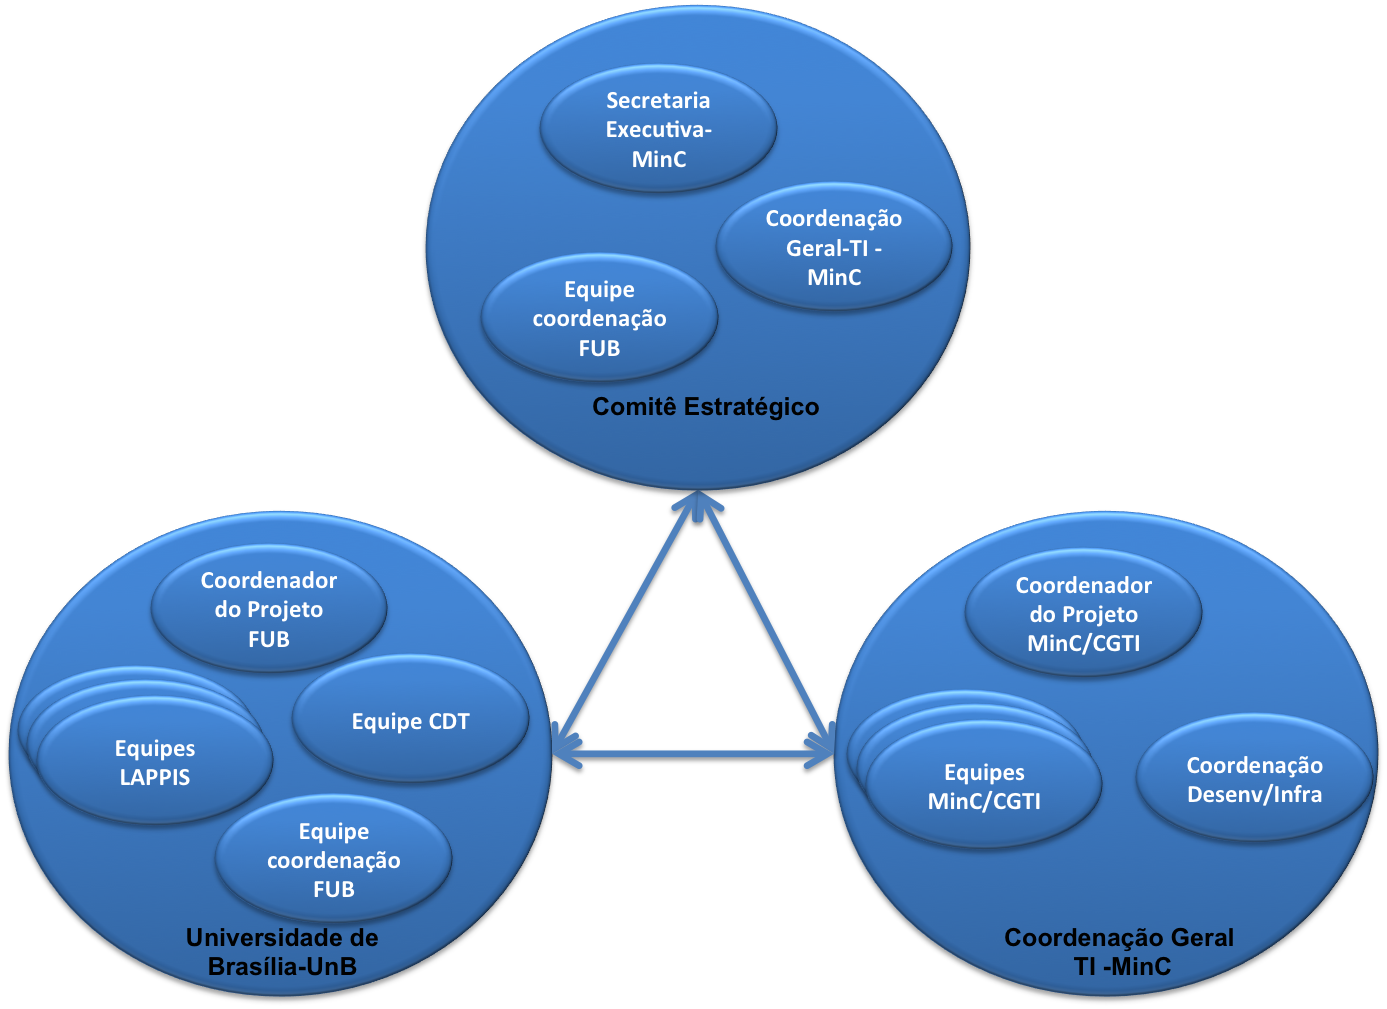
\includegraphics[keepaspectratio=true,scale=0.6]{figuras/Equipes_FUB-MINC.png}
\caption{Distribuição de equipes.}
\label{figura-equipes}
\end{figure}


A equipe do projeto é composto em sua maioria, cerca de 70\% da equipe total do projeto (respeitando a Resolução CONSUNI 17/2013), 
por professores e alunos de graduação e Pós graduação da Universidade de Brasília.  Os principais papéis envolvidos no projeto são:

\begin{itemize}
 \item \textbf{Professores Pesquisadores/Coordenadores}: dois professores do curso de Engenharia de Software estarão coordenando e
 orientando as pesquisas e desenvolvimento realizado ao longo do projeto.
 \item \textbf{Professores Pesquisadores}:  professores do curso de Engenharia de Software com experiência de mercado e pesquisa que ajudam 
 a consolidar o conhecimento dos alunos, além de orientá-los em termos de boas práticas e técnicas.
 \item \textbf{Alunos de Graduação Engenharia de Software}: serão responsáveis pelo desenvolvimento dos softwares desenvolvidos, 
 além execução da metodologia ágil e devops.
 \item \textbf{Desenvolvedores Comunidade de Software Livre}: são profissionais experientes envolvidos em comunidades de software livre 
 como desenvolvedores e design. Agregam no projeto ao compartilhar práticas, ferramentas, e conhecimento avançados no desenvolvimento
 de software livre e auxiliam na disseminação do conhecimento da equipe.  
\end{itemize}

Propõe-se a constituição de um comitê estratégico, composto por representantes da FUB e do MinC para garantir que as acões do projeto estejam alinhadas com os objetivos estratégicos do MinC.

As equipes técnicas serão formadas por engenheiros de software e artistas-designers, na sua maioria representadas por alunos da graduação em Engenharia de Software da UnB-Gama, que terão sua formação complementada por meio da oportunidade de participarem como protagonistas em um projeto desta magnitude durante sua formação. As equipes possuem diferentes experiências e qualificações, adequadas a dinâmica e complexidade do projeto.

A transferência de tecnologias e do conhecimento se dará primeiro pela interação direta entre bolsistas e pesquisadores do projeto e servidores da MinC/CGTEC, inclusive nas decisões de escolhas técnicas, formas de processo, metodologias. A apresentação de resultados será feita na forma de seminários para apresentação e discussão dos protótipos intermediários e finais, atendendo os normativos vigentes desta cooperação. Também ocorrerão oficinas técnicas de capacitação dos servidores e técnicos do MinC/CGTEC.



\subsection{Coordenadores}

\textbf{Profa. Carla Rocha Aguiar (Faculdade do Gama, UnB)}, Coordenadora Principal

Professora Adjunta do curso de Engenharia de Software. Graduada em Engenharia Mecatrônica pela Universidade de Brasília (UnB).
Doutorado em Ciência da Computação pelo Laboratoire d'Informatique Robotique et de Microélectronique de Montpellier (LIRMM). 
Principais produções
acadêmicas são em processamento (usando aprendizagem de máquina) de imagens de profundidade (Range Images) para o registro de modelos 3D e
restauração de obras de arte digital. 
Trabalho de doutorado fez parte do projeto de Pesquisa EROS3D, uma colaboração entre diversos laboratórios franceses, o museu do 
Louvre e o C2RMF (Centro de Pesquisa e de restauração dos museus da França). Participou de projeto de pesquisa sobre restauração
de obras de arte digital, parceria com o grupo Camera Culture (Media Lab, MIT).
Coordenadora do Laboratório Avançado em Produção, Pesquisa e Inovação em Software desde fevereiro 2017. 
Experiência em coordenação de projeto de pesquisa em colaboração com a Empresa Toledo S.A., via lei da informática. 


\textbf{Prof. Fábio Macêdo Mendes (Faculdade do Gama, UnB)}, Vice-coordenador 

Professor Adjunto do curso de Engenharia de Software. Graduado em Bacharelado em Física pela Universidade de  Brasília (UnB).
Doutorado e Mestrado em Física Matemática pelo Instituto de Física da Universidade de Brasília. Coordenador do LAPPIS desde fevereiro de 2017.
Principais contribuições acadêmicas na área do projeto são em gamificação em educação, modelos de clusterização, aprendizado de máquina,
estatística Bayesiana e processos Gaussianos. Também é contribuidor de vários projetos de software livre na comunidade Python, e em particular
coordena as iniciativas o Pytuguês, FGAme e o Codeschool.






% \section{Apresentação do Convenente}
% \label{convenente}
% 
% Para a realização do projeto, a Coordenação Geral de Tecnologia da Informação (CGTI) optou pela 
% cooperação com duas unidades acadêmicas da Fundação Universidade de Brasília (FUB), com o apoio do XXXXXXXXXX,
% de modo a utilizar pesquisas aplicadas e transferência de tecnologias e de conhecimento em temas avançados relativos ao
% projeto.
% 
% % LAPPIS
% O Laboratório Avançado de Produção, Pesquisa \& Inovação em Software (LAPPIS),
% localizado na Faculdade UnB Gama (FGA) foi criado em 2012 e foi concebido para
% atuar em áreas tecnológicas desde sistemas de informação até os sistemas
% embarcados, em especial, objetivando as oportunidades de pesquisas teóricas e
% aplicadas.
% %
% Em que pese sua recente criação, o laboratório, possui cooperações em andamento
% e concluídas com os segmentos da Administração Pública e Iniciativa Privada.
% Cabe ressaltar projetos já realizados com a Presidência República em parceria
% com o Serpro, Positivo Informática S/A, além da colaboração na evolução de
% diversas ferramentas de software livre.
% %
% O LAPPIS tem como objetivo contribuir com o desenvolvimento de projetos de
% software ao passo que complementamos a formação de Engenheiros de Software
% (capazes de lidar com problemas ao pensar em soluções computacionais e
% implamentá-las efetivamente), por meio de Métodos Ágeis, Software Livre,
% Segurança e Trabalho colaborativo centrado nas pessoas.
% %
% Com isso, oferece aos alunos de graduação em Engenharia de Software a
% oportunidade de aplicar os conceitos e as tecnologias em um ambiente produção
% de software real, sob orientação de professores especialistas nas áreas dos
% projetos do laboratório. Além da sua atuação na Faculdade UnB Gama, o LAPPIS
% tem uma parceria de colaboração com o Centro de Difusão de Tecnologia e
% Conhecimento, que é um projeto iniciado em Agosto de 2004, com a proposta de
% união de esforços entre o setor público e as universidades que fazem parte do
% estado com objetivo de ampliar o conhecimento da sociedade no uso do software
% livre.
% %
% O CDTC é um projeto de intenso impacto social, ampliando as liberdades
% individuais com o acesso da tecnologia pela sociedade, tendo ainda o estado uma
% grande economia de recursos a partir do usos de licenciamentos livres,
% permitindo assim que a economia com os recursos despendidos anualmente em
% licenças proprietárias de softwares, garanta o aquecimento de um mercado
% emergente, permitindo o acesso e apropriação tecnológica pelo próprio mercado
% nacional. Com o CDTC como parceiro, além do laboratório fisicamente localizado
% na UnB-Gama, o LAPPIS conta com um espaço físico, com excelente estrutura para
% as reuniões e desenvolvimento de projetos, no Campus da UnB Darcy Ribeiro.
% 
